\section{Example: Randomized Quicksort}

% New slide: QuickSort vs Randomized QuickSort steps
\begin{frame}{QuickSort vs Randomized QuickSort}
  \textbf{QuickSort:}
  \begin{enumerate}
    \item Pick a pivot element from the array \parencite{10.1093/comjnl/5.1.10}
    \item Split array into 3 subarrays: those smaller than pivot, those larger than pivot, and the pivot itself
    \item Recursively sort the subarrays, and concatenate them
  \end{enumerate}
  \vspace{1em}
  \textbf{Randomized QuickSort:}
  \begin{enumerate}
    \item Pick a pivot element \textbf{uniformly at random} from the array \parencite{motwani1995randomized}
    \item Split array into 3 subarrays: those smaller than pivot, those larger than pivot, and the pivot itself
    \item Recursively sort the subarrays, and concatenate them
  \end{enumerate}
\end{frame}

% New slide: Worst-case for QuickSort
\begin{frame}{Example: Randomized Quicksort}
  \textbf{Recall:} QuickSort can take $\Omega(n^2)$ time to sort an array of size $n$ \parencite{359631}
\end{frame}

% New slide: Theorem and expectation for Randomized QuickSort
\begin{frame}{Randomized QuickSort: Expected Runtime}
  \textbf{Theorem}
  \begin{block}{}
    Randomized QuickSort sorts a given array of length $n$ in $O(n \log n)$ expected time. \parencite{journals/acta/Sedgewick77}
  \end{block}
  \vspace{1em}
  \textbf{Note:} On every input, randomized QuickSort takes $O(n \log n)$ time in expectation. On every input, it may take $\Omega(n^2)$ time with some small probability.
\end{frame}

\subsection{Step-by-Step Execution}
\begin{frame}{Randomized Quicksort: Step 1 (Initial Array)}
  % Use columns for top-aligned split layout
  \begin{columns}[t]
    \column{0.6\textwidth}
    Consider the array:
    \[
      \renewcommand{\arraystretch}{1.5}
      \begin{array}{|c|c|c|c|c|c|c|c|}
        \hline
        15 & 3 & 1 & 10 & 9 & 0 & 6 & 4 \\
        \hline
      \end{array}
    \]
  \end{columns}
\end{frame}

\begin{frame}{Randomized Quicksort: Step 1.1 (Pivot Chosen)}
  % Use columns for top-aligned split layout
  \begin{columns}[t]
    \column{0.6\textwidth}
    Suppose the random pivot chosen is \textcolor{red}{10} (at index 3):
    \[
      \renewcommand{\arraystretch}{1.5}
      \begin{array}{|c|c|c|c|c|c|c|c|}
        \hline
        15 & 3 & 1 & \cellcolor{red!20}\textcolor{red}{10} & 9 & 0 & 6 & 4 \\
        \hline
      \end{array}
    \]

    \column{0.38\textwidth}
    \begin{minipage}[t]{\linewidth}
      \vspace{0pt}
      \begin{center}
        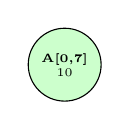
\begin{tikzpicture}[
          scale=0.85,
          transform shape,
          level distance=1.5cm,
          level 1/.style={sibling distance=3.0cm},
          level 2/.style={sibling distance=2.0cm},
          level 3/.style={sibling distance=1.2cm},
          every node/.style={font=\tiny}
        ]
          \node[circle, draw, fill=green!20, minimum size=1cm, align=center] (root) {
            \textbf{A[0,7]} \\
            10
          };
        \end{tikzpicture}
      \end{center}
    \end{minipage}
  \end{columns}
\end{frame}
% Step 2: Partitioning around 10
\begin{frame}{Randomized Quicksort: Step 2 (Partitioning Around Pivot 10)}
  % Use columns for top-aligned split layout
  \begin{columns}[t]
    \column{0.6\textwidth}
    After selecting pivot 10, we partition the array:
    \begin{itemize}
      \item \textcolor{green!60!black}{Left:} 4, 3, 1, 9, 0, 6 (elements before pivot position)
      \item \textcolor{red}{Middle:} 10 (pivot)
      \item \textcolor{blue}{Right:} 15 (element after pivot position)
    \end{itemize}

    After partitioning:
    \[
      \renewcommand{\arraystretch}{1.5}
      \begin{array}{|c|c|c|c|c|c|c|c|}
        \hline
        \cellcolor{green!20}\textcolor{green!60!black}{4} & \cellcolor{green!20}\textcolor{green!60!black}{3} & \cellcolor{green!20}\textcolor{green!60!black}{1} & \cellcolor{green!20}\textcolor{green!60!black}{9} & \cellcolor{green!20}\textcolor{green!60!black}{0} & \cellcolor{green!20}\textcolor{green!60!black}{6} & \cellcolor{red!20}\textcolor{red}{10} & 15 \\
        \hline
      \end{array}
    \]

    \column{0.38\textwidth}
    \begin{minipage}[t]{\linewidth}
      \vspace{0pt}
      \begin{center}
        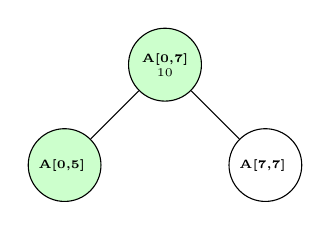
\begin{tikzpicture}[
          scale=0.85,
          transform shape,
          level distance=1.5cm,
          level 1/.style={sibling distance=3.0cm},
          level 2/.style={sibling distance=2.0cm},
          level 3/.style={sibling distance=1.2cm},
          every node/.style={font=\tiny}
        ]
          % Root node
          \node[circle, draw, fill=green!20, minimum size=1cm, align=center] (root) {
            \textbf{A[0,7]} \\
            10
          }
          % Left child
          child {node[circle, draw, fill=green!20, minimum size=1cm, align=center] {
                  \textbf{A[0,5]}
                }}
          % Right child
          child {node[circle, draw, fill=white, minimum size=1cm, align=center] {
                  \textbf{A[7,7]}
                }};
        \end{tikzpicture}
      \end{center}
    \end{minipage}
  \end{columns}
\end{frame}

% Step 3: Recurse Left [A[0,5]], Pivot 4
\begin{frame}{Randomized Quicksort: Step 3 (Recurse Left [A[0,5]], Pivot 4)}
  % Use columns for top-aligned split layout
  \begin{columns}[t]
    \column{0.6\textwidth}
    Recurse on the left subarray:
    \\[0.5em]
    Let's choose a random pivot, say 4.
    \[
      \renewcommand{\arraystretch}{1.5}
      \begin{array}{|c|c|c|c|c|c|}
        \hline
        \cellcolor{red!20}\textcolor{red}{4} & 3 & 1 & 9 & 0 & 6 \\
        \hline
      \end{array}
    \]

    \column{0.38\textwidth}
    \begin{minipage}[t]{\linewidth}
      \vspace{0pt}
      \begin{center}
        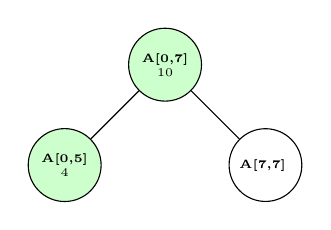
\begin{tikzpicture}[
          scale=0.85,
          transform shape,
          level distance=1.5cm,
          level 1/.style={sibling distance=3.0cm},
          level 2/.style={sibling distance=2.0cm},
          level 3/.style={sibling distance=1.2cm},
          every node/.style={font=\tiny}
        ]
          % Root node
          \node[circle, draw, fill=green!20, minimum size=1cm, align=center] (root) {
            \textbf{A[0,7]} \\
            10
          }
          % Left child
          child {node[circle, draw, fill=green!20, minimum size=1cm, align=center] {
                  \textbf{A[0,5]} \\
                  4
                }}
          % Right child
          child {node[circle, draw, fill=white, minimum size=1cm, align=center] {
                  \textbf{A[7,7]}
                }};
        \end{tikzpicture}
      \end{center}
    \end{minipage}
  \end{columns}
\end{frame}

% Step 3.1: Partition Left [A[0,5]] Around 4
\begin{frame}{Randomized Quicksort: Step 3.1 (Partition Left [A[0,5]] Around 4)}
  % Use columns for top-aligned split layout
  \begin{columns}[t]
    \column{0.6\textwidth}
    After partitioning the left subarray:
    \[
      \renewcommand{\arraystretch}{1.5}
      \begin{array}{|c|c|c|c|c|c|}
        \hline
        \cellcolor{green!20}\textcolor{green!60!black}{0} & \cellcolor{green!20}\textcolor{green!60!black}{3} & \cellcolor{green!20}\textcolor{green!60!black}{1} & \cellcolor{red!20}\textcolor{red}{4} & 9 & 6 \\
        \hline
      \end{array}
    \]
    Partition:
    \begin{itemize}
      \item \textcolor{green!60!black}{Left:} 0, 3, 1 (elements before pivot)
      \item \textcolor{red}{Middle:} 4 (pivot)
      \item \textcolor{blue}{Right:} 9, 6 (elements after pivot)
    \end{itemize}

    \column{0.38\textwidth}
    \begin{minipage}[t]{\linewidth}
      \vspace{0pt}
      \begin{center}
        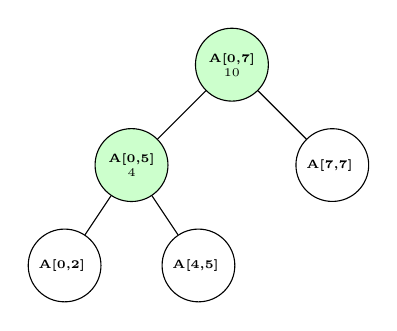
\begin{tikzpicture}[
          scale=0.85,
          transform shape,
          level distance=1.5cm,
          level 1/.style={sibling distance=3.0cm},
          level 2/.style={sibling distance=2.0cm},
          level 3/.style={sibling distance=1.2cm},
          every node/.style={font=\tiny}
        ]
          % Root node
          \node[circle, draw, fill=green!20, minimum size=1cm, align=center] (root) {
            \textbf{A[0,7]} \\
            10
          }
          % Left child
          child {node[circle, draw, fill=green!20, minimum size=1cm, align=center] {
                  \textbf{A[0,5]} \\
                  4
                }
              child {node[circle, draw, fill=white, minimum size=1cm, align=center] {
                      \textbf{A[0,2]}
                    }}
              child {node[circle, draw, fill=white, minimum size=1cm, align=center] {
                      \textbf{A[4,5]}
                    }}
            }
          % Right child
          child {node[circle, draw, fill=white, minimum size=1cm, align=center] {
                  \textbf{A[7,7]}
                }};
        \end{tikzpicture}
      \end{center}
    \end{minipage}
  \end{columns}
\end{frame}

% Step 3.1.1: Recurse Left [A[0,2]], Pivot 0
\begin{frame}{Randomized Quicksort: Step 3.1.1 (Recurse Left [A[0,2]], Pivot 0)}
  % Use columns for top-aligned split layout
  \begin{columns}[t]
    \column{0.6\textwidth}
    Recurse on the left subarray:
    \\[0.5em]
    Let's choose a random pivot, say 0.
    \[
      \renewcommand{\arraystretch}{1.5}
      \begin{array}{|c|c|c|}
        \hline
        \cellcolor{red!20}\textcolor{red}{0} & 3 & 1 \\
        \hline
      \end{array}
    \]

    \column{0.38\textwidth}
    \begin{minipage}[t]{\linewidth}
      \vspace{0pt}
      \begin{center}
        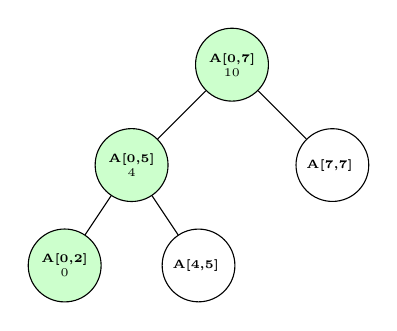
\begin{tikzpicture}[
          scale=0.85,
          transform shape,
          level distance=1.5cm,
          level 1/.style={sibling distance=3.0cm},
          level 2/.style={sibling distance=2.0cm},
          level 3/.style={sibling distance=1.2cm},
          every node/.style={font=\tiny}
        ]
          % Root node
          \node[circle, draw, fill=green!20, minimum size=1cm, align=center] (root) {
            \textbf{A[0,7]} \\
            10
          }
          % Left child
          child {node[circle, draw, fill=green!20, minimum size=1cm, align=center] {
                  \textbf{A[0,5]} \\
                  4
                }
              child {node[circle, draw, fill=green!20, minimum size=1cm, align=center] {
                      \textbf{A[0,2]}\\
                      0
                    }}
              child {node[circle, draw, fill=white, minimum size=1cm, align=center] {
                      \textbf{A[4,5]}
                    }}
            }
          % Right child
          child {node[circle, draw, fill=white, minimum size=1cm, align=center] {
                  \textbf{A[7,7]}
                }
            };
        \end{tikzpicture}
      \end{center}
    \end{minipage}
  \end{columns}
\end{frame}

% Step 3.1.1.1: Partition Left [A[0,2]] Around 0
\begin{frame}{Randomized Quicksort: Step 3.1.1.1 (Partition Left [A[0,2]] Around 0)}
  % Use columns for top-aligned split layout
  \begin{columns}[t]
    \column{0.6\textwidth}
    After partitioning the left subarray:
    \[
      \renewcommand{\arraystretch}{1.5}
      \begin{array}{|c|c|c|}
        \hline
        \cellcolor{red!20}\textcolor{red}{0} & 3 & 1 \\
        \hline
      \end{array}
    \]
    Partition:
    \begin{itemize}
      \item \textcolor{green!60!black}{Left:} (empty)
      \item \textcolor{red}{Middle:} 0 (pivot)
      \item \textcolor{blue}{Right:} 3, 1 (elements after pivot)
    \end{itemize}

    \column{0.38\textwidth}
    \begin{minipage}[t]{\linewidth}
      \vspace{0pt}
      \begin{center}
        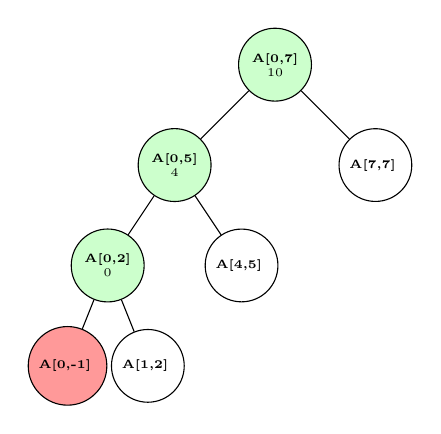
\begin{tikzpicture}[
          scale=0.85,
          transform shape,
          level distance=1.5cm,
          level 1/.style={sibling distance=3.0cm},
          level 2/.style={sibling distance=2.0cm},
          level 3/.style={sibling distance=1.2cm},
          every node/.style={font=\tiny}
        ]
          % Root node
          \node[circle, draw, fill=green!20, minimum size=1cm, align=center] (root) {
            \textbf{A[0,7]} \\
            10
          }
          % Left child
          child {node[circle, draw, fill=green!20, minimum size=1cm, align=center] {
                  \textbf{A[0,5]} \\
                  4
                }
              child {node[circle, draw, fill=green!20, minimum size=1cm, align=center] {
                      \textbf{A[0,2]}\\
                      0
                    }
                  child {node[circle, draw, fill=red!40, minimum size=1cm, align=center] {
                          \textbf{A[0,-1]}
                        }}
                  child {node[circle, draw, fill=white, minimum size=1cm, align=center] {
                          \textbf{A[1,2]}
                        }}
                }
              child {node[circle, draw, fill=white, minimum size=1cm, align=center] {
                      \textbf{A[4,5]}
                    }}
            }
          % Right child
          child {node[circle, draw, fill=white, minimum size=1cm, align=center] {
                  \textbf{A[7,7]}
                }
            };
        \end{tikzpicture}
      \end{center}
    \end{minipage}
  \end{columns}
\end{frame}

\begin{frame}{Randomized Quicksort: Step 3.1.1.2 (Recurse Right [A[1,2]], Pivot 3)}
  % Use columns for top-aligned split layout
  \begin{columns}[t]
    \column{0.6\textwidth}
    Recurse on the right subarray:
    \\[0.5em]
    Let's choose a random pivot, say 3.
    \[
      \renewcommand{\arraystretch}{1.5}
      \begin{array}{|c|c|}
        \hline
        \cellcolor{red!20}\textcolor{red}{3} & 1 \\
        \hline
      \end{array}
    \]

    \column{0.38\textwidth}
    \begin{minipage}[t]{\linewidth}
      \vspace{0pt}
      \begin{center}
        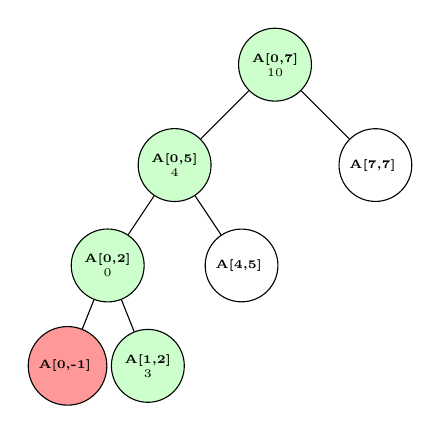
\begin{tikzpicture}[
          scale=0.85,
          transform shape,
          level distance=1.5cm,
          level 1/.style={sibling distance=3.0cm},
          level 2/.style={sibling distance=2.0cm},
          level 3/.style={sibling distance=1.2cm},
          every node/.style={font=\tiny}
        ]
          % Root node
          \node[circle, draw, fill=green!20, minimum size=1cm, align=center] (root) {
            \textbf{A[0,7]} \\
            10
          }
          % Left child
          child {node[circle, draw, fill=green!20, minimum size=1cm, align=center] {
                  \textbf{A[0,5]} \\
                  4
                }
              child {node[circle, draw, fill=green!20, minimum size=1cm, align=center] {
                      \textbf{A[0,2]}\\
                      0
                    }
                  child {node[circle, draw, fill=red!40, minimum size=1cm, align=center] {
                          \textbf{A[0,-1]}
                        }}
                  child {node[circle, draw, fill=green!20, minimum size=1cm, align=center] {
                          \textbf{A[1,2]}\\
                          3
                        }
                    }
                }
              child {node[circle, draw, fill=white, minimum size=1cm, align=center] {
                      \textbf{A[4,5]}
                    }}
            }
          % Right child
          child {node[circle, draw, fill=white, minimum size=1cm, align=center] {
                  \textbf{A[7,7]}
                }
            };
        \end{tikzpicture}
      \end{center}
    \end{minipage}
  \end{columns}
\end{frame}

% Step 3.1.1.2.1: Partition [A[1,2]] Around 3
\begin{frame}{Randomized Quicksort: Step 3.1.1.2.1 (Partition [A[1,2]] Around 3)}
  % Use columns for top-aligned split layout
  \begin{columns}[t]
    \column{0.6\textwidth}
    After partitioning the left subarray:
    \[
      \renewcommand{\arraystretch}{1.5}
      \begin{array}{|c|c|c|}
        \hline
        1 & \cellcolor{red!20}\textcolor{red}{3} \\
        \hline
      \end{array}
    \]
    Partition:
    \begin{itemize}
      \item \textcolor{green!60!black}{Left:} 1 (element before pivot)
      \item \textcolor{red}{Middle:} 3 (pivot)
      \item \textcolor{blue}{Right:} (empty)
    \end{itemize}

    \column{0.38\textwidth}
    \begin{minipage}[t]{\linewidth}
      \vspace{0pt} % Ensures true top alignment
      \begin{center}

        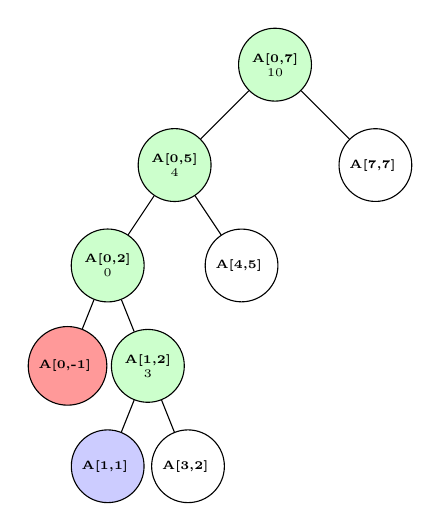
\begin{tikzpicture}[
          scale=0.85,
          transform shape,
          level distance=1.5cm,
          level 1/.style={sibling distance=3.0cm},
          level 2/.style={sibling distance=2.0cm},
          level 3/.style={sibling distance=1.2cm},
          every node/.style={font=\tiny}
        ]
          % Root node
          \node[circle, draw, fill=green!20, minimum size=1cm, align=center] (root) {
            \textbf{A[0,7]} \\
            10
          }
          % Left child
          child {node[circle, draw, fill=green!20, minimum size=1cm, align=center] {
                  \textbf{A[0,5]} \\
                  4
                }
              child {node[circle, draw, fill=green!20, minimum size=1cm, align=center] {
                      \textbf{A[0,2]}\\
                      0
                    }
                  child {node[circle, draw, fill=red!40, minimum size=1cm, align=center] {
                          \textbf{A[0,-1]}
                        }}
                  child {node[circle, draw, fill=green!20, minimum size=1cm, align=center] {
                          \textbf{A[1,2]}\\
                          3
                        }
                      child {node[circle, draw, fill=blue!20, minimum size=1cm, align=center] {
                              \textbf{A[1,1]}
                            }
                        }
                      child {node[circle, draw, fill=white, minimum size=1cm, align=center] {
                              \textbf{A[3,2]}
                            }
                        }
                    }
                }
              child {node[circle, draw, fill=white, minimum size=1cm, align=center] {
                      \textbf{A[4,5]}
                    }}
            }
          % Right child
          child {node[circle, draw, fill=white, minimum size=1cm, align=center] {
                  \textbf{A[7,7]}
                }
            };
        \end{tikzpicture}
      \end{center}
    \end{minipage}
  \end{columns}
\end{frame}

% Step 3.1.1.2.1.1: Recurse Left [A[1,1]], Done
\begin{frame}{Randomized Quicksort: Step 3.1.1.2.1.1 (Recurse Left [A[1,1]], Done)}
  \begin{columns}[t]
    \column{0.6\textwidth}
    After partitioning the left subarray:
    \[
      \renewcommand{\arraystretch}{1.5}
      \begin{array}{|c|c|c|}
        \hline
        \cellcolor{green!20}{1} \\
        \hline
      \end{array}
    \]

    Partition:
    \begin{itemize}
      \item \textcolor{green!60!black}{Left:} (empty)
      \item \textcolor{red}{Middle:} 1 (pivot)
      \item \textcolor{blue}{Right:} (empty)
    \end{itemize}
    Single element subarray, done, return.
    \column{0.38\textwidth}
    \begin{minipage}[t]{\linewidth}
      \vspace{0pt} % Ensures true top alignment
      \begin{center}

        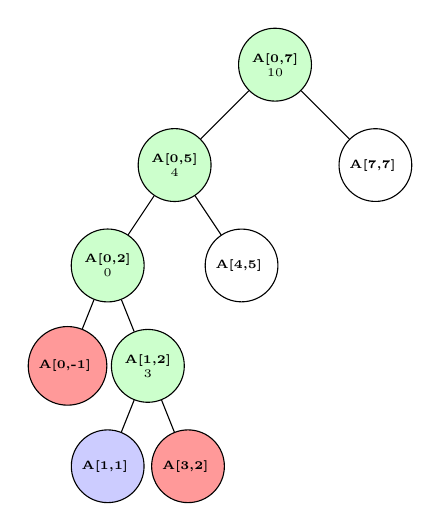
\begin{tikzpicture}[
          scale=0.85,
          transform shape,
          level distance=1.5cm,
          level 1/.style={sibling distance=3.0cm},
          level 2/.style={sibling distance=2.0cm},
          level 3/.style={sibling distance=1.2cm},
          every node/.style={font=\tiny}
        ]
          % Root node
          \node[circle, draw, fill=green!20, minimum size=1cm, align=center] (root) {
            \textbf{A[0,7]} \\
            10
          }
          % Left child
          child {node[circle, draw, fill=green!20, minimum size=1cm, align=center] {
                  \textbf{A[0,5]} \\
                  4
                }
              child {node[circle, draw, fill=green!20, minimum size=1cm, align=center] {
                      \textbf{A[0,2]}\\
                      0
                    }
                  child {node[circle, draw, fill=red!40, minimum size=1cm, align=center] {
                          \textbf{A[0,-1]}
                        }}
                  child {node[circle, draw, fill=green!20, minimum size=1cm, align=center] {
                          \textbf{A[1,2]}\\
                          3
                        }
                      child {node[circle, draw, fill=blue!20, minimum size=1cm, align=center] {
                              \textbf{A[1,1]}
                            }
                        }
                      child {node[circle, draw, fill=red!40, minimum size=1cm, align=center] {
                              \textbf{A[3,2]}
                            }
                        }
                    }
                }
              child {node[circle, draw, fill=white, minimum size=1cm, align=center] {
                      \textbf{A[4,5]}
                    }}
            }
          % Right child
          child {node[circle, draw, fill=white, minimum size=1cm, align=center] {
                  \textbf{A[7,7]}
                }
            };
        \end{tikzpicture}
      \end{center}
    \end{minipage}
  \end{columns}
\end{frame}

% Step 3.1.1.2.1.2: Recurse Right [A[3,2]], Done
\begin{frame}{Randomized Quicksort: Step 3.1.1.2.1.2 (Recurse Right [A[3,2]], Done)}
  \begin{columns}[t]
    \column{0.6\textwidth}
    Recurse on the right subarray $A[3,2]$ (empty, done).
    Return to parent call $A[1,2]$
    \column{0.38\textwidth}
    \begin{minipage}[t]{\linewidth}
      \vspace{0pt} % Ensures true top alignment
      \begin{center}

        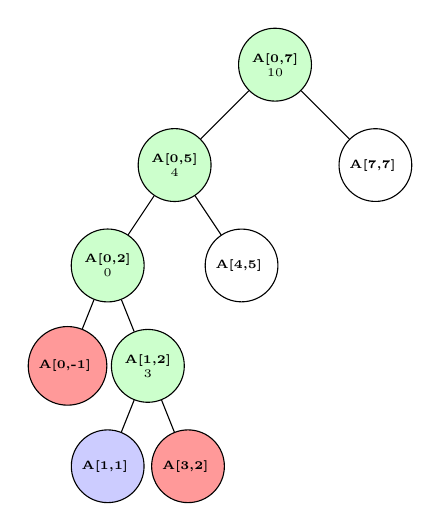
\begin{tikzpicture}[
          scale=0.85,
          transform shape,
          level distance=1.5cm,
          level 1/.style={sibling distance=3.0cm},
          level 2/.style={sibling distance=2.0cm},
          level 3/.style={sibling distance=1.2cm},
          every node/.style={font=\tiny}
        ]
          % Root node
          \node[circle, draw, fill=green!20, minimum size=1cm, align=center] (root) {
            \textbf{A[0,7]} \\
            10
          }
          % Left child
          child {node[circle, draw, fill=green!20, minimum size=1cm, align=center] {
                  \textbf{A[0,5]} \\
                  4
                }
              child {node[circle, draw, fill=green!20, minimum size=1cm, align=center] {
                      \textbf{A[0,2]}\\
                      0
                    }
                  child {node[circle, draw, fill=red!40, minimum size=1cm, align=center] {
                          \textbf{A[0,-1]}
                        }}
                  child {node[circle, draw, fill=green!20, minimum size=1cm, align=center] {
                          \textbf{A[1,2]}\\
                          3
                        }
                      child {node[circle, draw, fill=blue!20, minimum size=1cm, align=center] {
                              \textbf{A[1,1]}
                            }
                        }
                      child {node[circle, draw, fill=red!40, minimum size=1cm, align=center] {
                              \textbf{A[3,2]}
                            }
                        }
                    }
                }
              child {node[circle, draw, fill=white, minimum size=1cm, align=center] {
                      \textbf{A[4,5]}
                    }}
            }
          % Right child
          child {node[circle, draw, fill=white, minimum size=1cm, align=center] {
                  \textbf{A[7,7]}
                }
            };
        \end{tikzpicture}
      \end{center}
    \end{minipage}
  \end{columns}
\end{frame}

% Step 3.1.2: Return to [A[0,2]]
\begin{frame}{Randomized Quicksort: Step 3.1.2 (Return to [A[0,2]])}
  \begin{columns}[t]
    \column{0.6\textwidth}
    Return to parent call $A[0,2]$
    \column{0.38\textwidth}
    \begin{minipage}[t]{\linewidth}
      \vspace{0pt} % Ensures true top alignment
      \begin{center}

        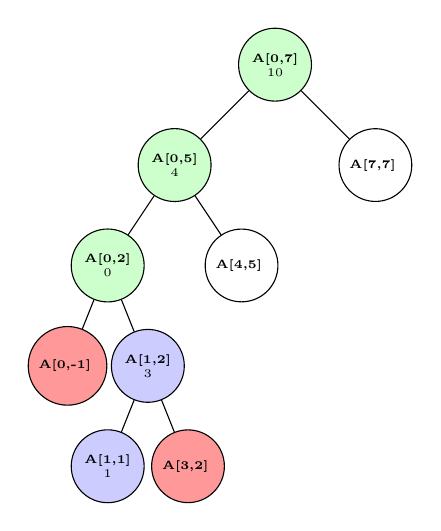
\begin{tikzpicture}[
          scale=0.85,
          transform shape,
          level distance=1.5cm,
          level 1/.style={sibling distance=3.0cm},
          level 2/.style={sibling distance=2.0cm},
          level 3/.style={sibling distance=1.2cm},
          every node/.style={font=\tiny}
        ]
          % Root node
          \node[circle, draw, fill=green!20, minimum size=1cm, align=center] (root) {
            \textbf{A[0,7]} \\
            10
          }
          % Left child
          child {node[circle, draw, fill=green!20, minimum size=1cm, align=center] {
                  \textbf{A[0,5]} \\
                  4
                }
              child {node[circle, draw, fill=green!20, minimum size=1cm, align=center] {
                      \textbf{A[0,2]}\\
                      0
                    }
                  child {node[circle, draw, fill=red!40, minimum size=1cm, align=center] {
                          \textbf{A[0,-1]}
                        }}
                  child {node[circle, draw, fill=blue!20, minimum size=1cm, align=center] {
                          \textbf{A[1,2]}\\
                          3
                        }
                      child {node[circle, draw, fill=blue!20, minimum size=1cm, align=center] {
                              \textbf{A[1,1]}\\
                              1
                            }
                        }
                      child {node[circle, draw, fill=red!40, minimum size=1cm, align=center] {
                              \textbf{A[3,2]}
                            }
                        }
                    }
                }
              child {node[circle, draw, fill=white, minimum size=1cm, align=center] {
                      \textbf{A[4,5]}
                    }}
            }
          % Right child
          child {node[circle, draw, fill=white, minimum size=1cm, align=center] {
                  \textbf{A[7,7]}
                }
            };
        \end{tikzpicture}
      \end{center}
    \end{minipage}
  \end{columns}
\end{frame}

% Step 3.2: Recurse Right [A[4,5]], Pivot 9
\begin{frame}{Randomized Quicksort: Step 3.2 (Recurse Right [A[4,5]], Pivot 9)}
  \begin{columns}[t]
    \column{0.6\textwidth}
    Recurse on the right subarray $A[4,5]$:
    \\[0.5em]
    Let's choose a random pivot, say 9.
    \[
      \renewcommand{\arraystretch}{1.5}
      \begin{array}{|c|c|}
        \hline
        \cellcolor{red!20}\textcolor{red}{9} & 6 \\
        \hline
      \end{array}
    \]

    \column{0.38\textwidth}
    \begin{minipage}[t]{\linewidth}
      \vspace{0pt} % Ensures true top alignment
      \begin{center}

        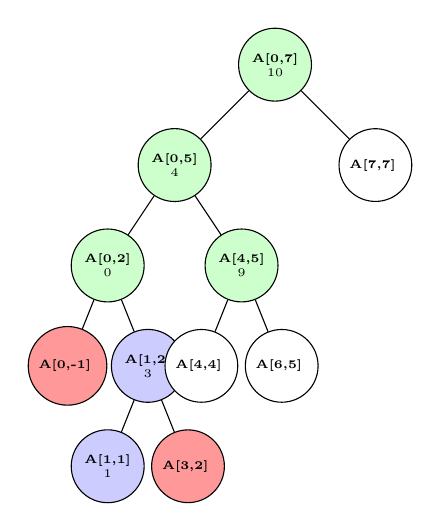
\begin{tikzpicture}[
          scale=0.85,
          transform shape,
          level distance=1.5cm,
          level 1/.style={sibling distance=3.0cm},
          level 2/.style={sibling distance=2.0cm},
          level 3/.style={sibling distance=1.2cm},
          every node/.style={font=\tiny}
        ]
          % Root node
          \node[circle, draw, fill=green!20, minimum size=1cm, align=center] (root) {
            \textbf{A[0,7]} \\
            10
          }
          % Left child
          child {node[circle, draw, fill=green!20, minimum size=1cm, align=center] {
                  \textbf{A[0,5]} \\
                  4
                }
              child {node[circle, draw, fill=green!20, minimum size=1cm, align=center] {
                      \textbf{A[0,2]}\\
                      0
                    }
                  child {node[circle, draw, fill=red!40, minimum size=1cm, align=center] {
                          \textbf{A[0,-1]}
                        }}
                  child {node[circle, draw, fill=blue!20, minimum size=1cm, align=center] {
                          \textbf{A[1,2]}\\
                          3
                        }
                      child {node[circle, draw, fill=blue!20, minimum size=1cm, align=center] {
                              \textbf{A[1,1]}\\
                              1
                            }
                        }
                      child {node[circle, draw, fill=red!40, minimum size=1cm, align=center] {
                              \textbf{A[3,2]}
                            }
                        }
                    }
                }
              child {node[circle, draw, fill=green!20, minimum size=1cm, align=center] {
                      \textbf{A[4,5]}\\
                      9
                    }
                    child {node[circle, draw, fill=white, minimum size=1cm, align=center] {
                    \textbf{A[4,4]}
                        }}
                  child {node[circle, draw, fill=white, minimum size=1cm, align=center] {
                      \textbf{A[6,5]}
                    }}
                  }
            }
          % Right child
          child {node[circle, draw, fill=white, minimum size=1cm, align=center] {
                  \textbf{A[7,7]}
                }
            };
        \end{tikzpicture}
      \end{center}
    \end{minipage}
  \end{columns}
\end{frame}

% Step 3.2.1: Partition [A[4,5]] Around 9
\begin{frame}{Randomized Quicksort: Step 3.2.1 (Partition [A[4,5]] Around 9)}
  \begin{columns}[t]
    \column{0.6\textwidth}
    Recurse on the right subarray $A[4,5]$:
    \\[0.5em]

    Suppose the random pivot is \textcolor{red}{9}:
    \[
      \renewcommand{\arraystretch}{1.5}
      \begin{array}{|c|c|}
        \hline
        6 & \cellcolor{red!20}\textcolor{red}{9} \\
        \hline
      \end{array}
    \]

    Partition:
    \begin{itemize}
      \item \textcolor{green!60!black}{Left:} 6 (element before pivot)
      \item \textcolor{red}{Middle:} 9 (pivot)
      \item \textcolor{blue}{Right:} (empty)
    \end{itemize}

    \column{0.38\textwidth}
    \begin{minipage}[t]{\linewidth}
      \vspace{0pt} % Ensures true top alignment
      \begin{center}

        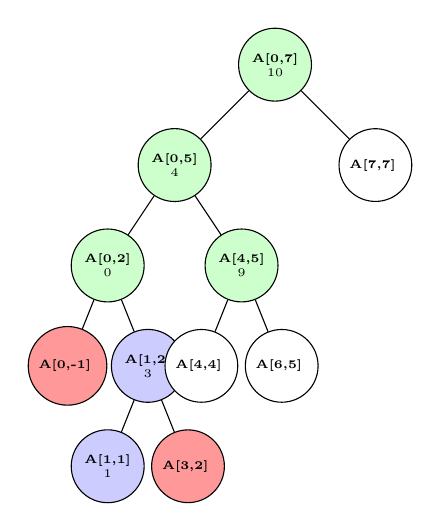
\begin{tikzpicture}[
          scale=0.85,
          transform shape,
          level distance=1.5cm,
          level 1/.style={sibling distance=3.0cm},
          level 2/.style={sibling distance=2.0cm},
          level 3/.style={sibling distance=1.2cm},
          every node/.style={font=\tiny}
        ]
          % Root node
          \node[circle, draw, fill=green!20, minimum size=1cm, align=center] (root) {
            \textbf{A[0,7]} \\
            10
          }
          % Left child
          child {node[circle, draw, fill=green!20, minimum size=1cm, align=center] {
                  \textbf{A[0,5]} \\
                  4
                }
              child {node[circle, draw, fill=green!20, minimum size=1cm, align=center] {
                      \textbf{A[0,2]}\\
                      0
                    }
                  child {node[circle, draw, fill=red!40, minimum size=1cm, align=center] {
                          \textbf{A[0,-1]}
                        }}
                  child {node[circle, draw, fill=blue!20, minimum size=1cm, align=center] {
                          \textbf{A[1,2]}\\
                          3
                        }
                      child {node[circle, draw, fill=blue!20, minimum size=1cm, align=center] {
                              \textbf{A[1,1]}\\
                              1
                            }
                        }
                      child {node[circle, draw, fill=red!40, minimum size=1cm, align=center] {
                              \textbf{A[3,2]}
                            }
                        }
                    }
                }
              child {node[circle, draw, fill=green!20, minimum size=1cm, align=center] {
                      \textbf{A[4,5]}\\
                      9
                    }
                  child {node[circle, draw, fill=white, minimum size=1cm, align=center] {
                          \textbf{A[4,4]}
                        }}
                  child {node[circle, draw, fill=white, minimum size=1cm, align=center] {
                          \textbf{A[6,5]}
                        }}
                }
            }
          % Right child
          child {node[circle, draw, fill=white, minimum size=1cm, align=center] {
                  \textbf{A[7,7]}
                }
            };
        \end{tikzpicture}
      \end{center}
    \end{minipage}
  \end{columns}
\end{frame}

% Step 3.2.1.1: Recurse Left [A[4,4]], Done
\begin{frame}{Randomized Quicksort: Step 3.2.1.1 (Recurse Left [A[4,4]], Done)}
  \begin{columns}[t]
    \column{0.6\textwidth}
    After partitioning the left subarray:
    \[
      \renewcommand{\arraystretch}{1.5}
      \begin{array}{|c|c|c|}
        \hline
        \cellcolor{green!20}{6} \\
        \hline
      \end{array}
    \]

    Partition:
    \begin{itemize}
      \item \textcolor{green!60!black}{Left:} (empty)
      \item \textcolor{red}{Middle:} 6 (pivot)
      \item \textcolor{blue}{Right:} (empty)
    \end{itemize}
    Single element subarray, done, return.
    \column{0.38\textwidth}
    \begin{minipage}[t]{\linewidth}
      \vspace{0pt} % Ensures true top alignment
      \begin{center}

        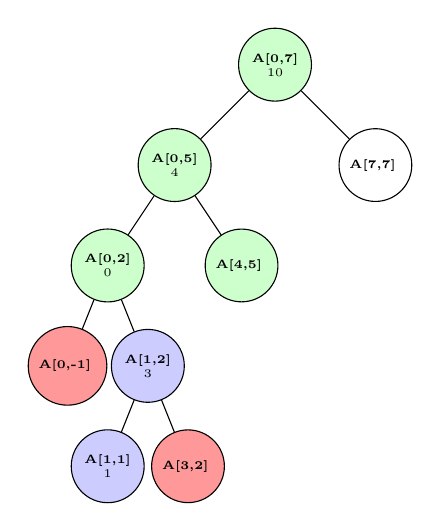
\begin{tikzpicture}[
          scale=0.85,
          transform shape,
          level distance=1.5cm,
          level 1/.style={sibling distance=3.0cm},
          level 2/.style={sibling distance=2.0cm},
          level 3/.style={sibling distance=1.2cm},
          every node/.style={font=\tiny}
        ]
          % Root node
          \node[circle, draw, fill=green!20, minimum size=1cm, align=center] (root) {
            \textbf{A[0,7]} \\
            10
          }
          % Left child
          child {node[circle, draw, fill=green!20, minimum size=1cm, align=center] {
                  \textbf{A[0,5]} \\
                  4
                }
              child {node[circle, draw, fill=green!20, minimum size=1cm, align=center] {
                      \textbf{A[0,2]}\\
                      0
                    }
                  child {node[circle, draw, fill=red!40, minimum size=1cm, align=center] {
                          \textbf{A[0,-1]}
                        }}
                  child {node[circle, draw, fill=blue!20, minimum size=1cm, align=center] {
                          \textbf{A[1,2]}\\
                          3
                        }
                      child {node[circle, draw, fill=blue!20, minimum size=1cm, align=center] {
                              \textbf{A[1,1]}\\
                              1
                            }
                        }
                      child {node[circle, draw, fill=red!40, minimum size=1cm, align=center] {
                              \textbf{A[3,2]}
                            }
                        }
                    }
                }
              child {node[circle, draw, fill=green!20, minimum size=1cm, align=center] {
                      \textbf{A[4,5]}
                      }}
            }
          % Right child
          child {node[circle, draw, fill=white, minimum size=1cm, align=center] {
                  \textbf{A[7,7]}
                }
            };
        \end{tikzpicture}
      \end{center}
    \end{minipage}
  \end{columns}
\end{frame}

% Step 3.2.1.2: Recurse Right [A[6,5]], Done
\begin{frame}{Randomized Quicksort: Step 3.2.1.2 (Recurse Right [A[6,5]], Done)}
  \begin{columns}[t]
    \column{0.6\textwidth}
    Recurse on the right subarray $A[6,5]$ (empty, done).
    Return to parent call $A[4,5]$\\
    Return to parent call $A[0,5]$\\
    \column{0.38\textwidth}
    \begin{minipage}[t]{\linewidth}
      \vspace{0pt} % Ensures true top alignment
      \begin{center}

        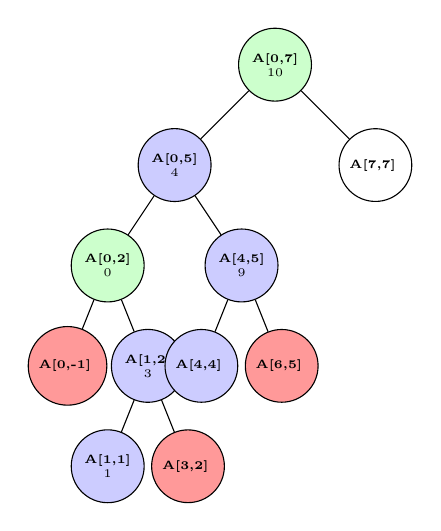
\begin{tikzpicture}[
          scale=0.85,
          transform shape,
          level distance=1.5cm,
          level 1/.style={sibling distance=3.0cm},
          level 2/.style={sibling distance=2.0cm},
          level 3/.style={sibling distance=1.2cm},
          every node/.style={font=\tiny}
        ]
          % Root node
          \node[circle, draw, fill=green!20, minimum size=1cm, align=center] (root) {
            \textbf{A[0,7]} \\
            10
          }
          % Left child
          child {node[circle, draw, fill=blue!20, minimum size=1cm, align=center] {
                  \textbf{A[0,5]} \\
                  4
                }
              child {node[circle, draw, fill=green!20, minimum size=1cm, align=center] {
                      \textbf{A[0,2]}\\
                      0
                    }
                  child {node[circle, draw, fill=red!40, minimum size=1cm, align=center] {
                          \textbf{A[0,-1]}
                        }}
                  child {node[circle, draw, fill=blue!20, minimum size=1cm, align=center] {
                          \textbf{A[1,2]}\\
                          3
                        }
                      child {node[circle, draw, fill=blue!20, minimum size=1cm, align=center] {
                              \textbf{A[1,1]}\\
                              1
                            }
                        }
                      child {node[circle, draw, fill=red!40, minimum size=1cm, align=center] {
                              \textbf{A[3,2]}
                            }
                        }
                    }
                }
              child {node[circle, draw, fill=blue!20, minimum size=1cm, align=center] {
                      \textbf{A[4,5]}\\
                      9
                    }
                  child {node[circle, draw, fill=blue!20, minimum size=1cm, align=center] {
                          \textbf{A[4,4]}
                        }}
                  child {node[circle, draw, fill=red!40, minimum size=1cm, align=center] {
                          \textbf{A[6,5]}
                        }}
                }
            }
          % Right child
          child {node[circle, draw, fill=white, minimum size=1cm, align=center] {
                  \textbf{A[7,7]}
                }
            };
        \end{tikzpicture}
      \end{center}
    \end{minipage}
  \end{columns}
\end{frame}

% Step 3.3: Recurse Right [A[7,7]], Done
\begin{frame}{Randomized Quicksort: Step 3.3 (Recurse Right [A[7,7]], Done)}
  \begin{columns}[t]
    \column{0.6\textwidth}
    Recurse on the right subarray $A[7,7]$
    After partitioning the right subarray:
    \[
      \renewcommand{\arraystretch}{1.5}
      \begin{array}{|c|c|c|}
        \hline
        \cellcolor{green!20}{1} \\
        \hline
      \end{array}
    \]

    Partition:
    \begin{itemize}
      \item \textcolor{green!60!black}{Left:} (empty)
      \item \textcolor{red}{Middle:} 1 (pivot)
      \item \textcolor{blue}{Right:} (empty)
    \end{itemize}
    Single element subarray, done, return.
    \column{0.38\textwidth}
    \begin{minipage}[t]{\linewidth}
      \vspace{0pt} % Ensures true top alignment
      \begin{center}

        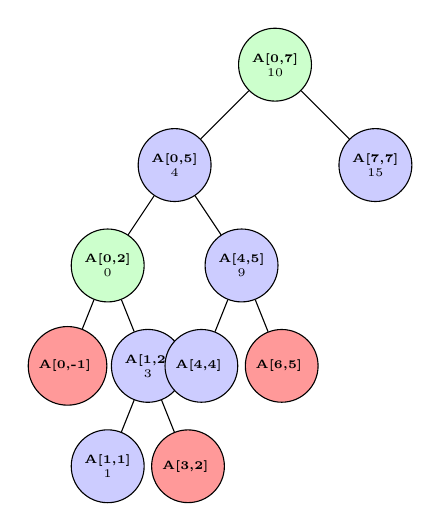
\begin{tikzpicture}[
          scale=0.85,
          transform shape,
          level distance=1.5cm,
          level 1/.style={sibling distance=3.0cm},
          level 2/.style={sibling distance=2.0cm},
          level 3/.style={sibling distance=1.2cm},
          every node/.style={font=\tiny}
        ]
          % Root node
          \node[circle, draw, fill=green!20, minimum size=1cm, align=center] (root) {
            \textbf{A[0,7]} \\
            10
          }
          % Left child
          child {node[circle, draw, fill=blue!20, minimum size=1cm, align=center] {
                  \textbf{A[0,5]} \\
                  4
                }
              child {node[circle, draw, fill=green!20, minimum size=1cm, align=center] {
                      \textbf{A[0,2]}\\
                      0
                    }
                  child {node[circle, draw, fill=red!40, minimum size=1cm, align=center] {
                          \textbf{A[0,-1]}
                        }}
                  child {node[circle, draw, fill=blue!20, minimum size=1cm, align=center] {
                          \textbf{A[1,2]}\\
                          3
                        }
                      child {node[circle, draw, fill=blue!20, minimum size=1cm, align=center] {
                              \textbf{A[1,1]}\\
                              1
                            }
                        }
                      child {node[circle, draw, fill=red!40, minimum size=1cm, align=center] {
                              \textbf{A[3,2]}
                            }
                        }
                    }
                }
              child {node[circle, draw, fill=blue!20, minimum size=1cm, align=center] {
                      \textbf{A[4,5]}\\
                      9
                    }
                  child {node[circle, draw, fill=blue!20, minimum size=1cm, align=center] {
                          \textbf{A[4,4]}
                        }}
                  child {node[circle, draw, fill=red!40, minimum size=1cm, align=center] {
                          \textbf{A[6,5]}
                        }}
                }
            }
          % Right child
          child {node[circle, draw, fill=blue!20, minimum size=1cm, align=center] {
                  \textbf{A[7,7]} \\
                  15
                }
            };
        \end{tikzpicture}
      \end{center}
    \end{minipage}
  \end{columns}
\end{frame}

% Step 4: Final Sorted Array
\begin{frame}{Randomized Quicksort: Step 4 (Final Sorted Array)}
  The final sorted array is:
  \[
    \renewcommand{\arraystretch}{1.5}
    \begin{array}{|c|c|c|c|c|c|c|c|}
      \hline
      0 & 1 & 3 & 4 & 6 & 9 & 10 & 15 \\
      \hline
    \end{array}
  \]
\end{frame}

\begin{frame}{Quicksort Time Complexity}
  \begin{itemize}
    \item \textbf{Worst-case:} $O(n^2)$
    \item \textbf{Best-case:} $O(n \log n)$
    \item \textbf{Expected:} $O(n \log n)$ (randomized)
  \end{itemize}
\end{frame}
